\documentclass[a4paper,11pt]{ujreport}
%%【PostScript, JPEG, PNG等の画像の貼り込み】
%% 利用するパッケージを選んでコメントアウトしてください.
\usepackage{graphicx} % for 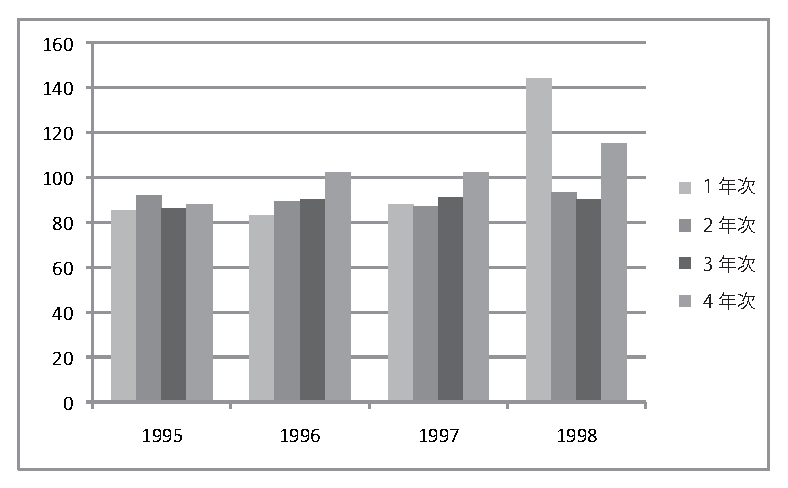
\includegraphics[width=3cm]{sample.eps}
\usepackage{epsfig} % for 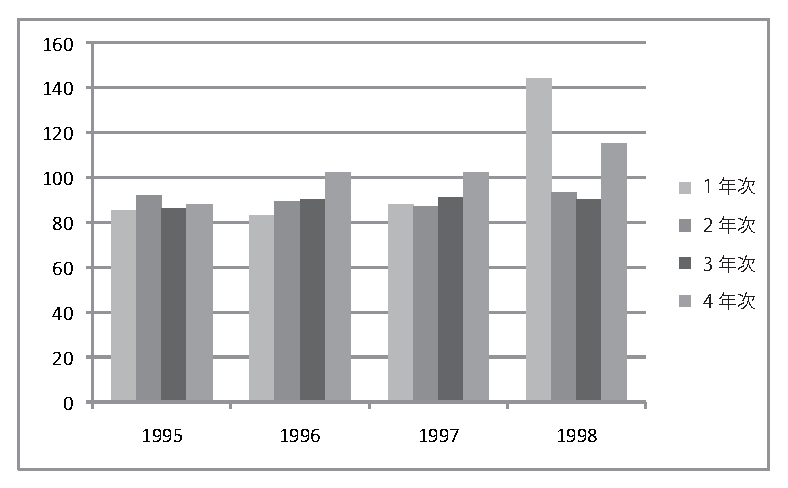
\psfig{file=sample.eps,width=3cm}
%\usepackage{epsf} % for \epsfile{file=sample.eps,scale=0.6}
%\usepackage{epsbox} % for \epsfile{file=sample.eps,scale=0.6}
\usepackage{/Users/takagihayata/workspace/materialize-mongodb/paper/mast/class/mediabb} % for pdf

\usepackage{times} % use Times Font instead of Computer Modern
% \usepackage{listings} % for soursecode
% \usepackage{plistings} % for soursecode
\usepackage{/Users/takagihayata/workspace/materialize-mongodb/paper/mast/class/docmute} % texファイル分割用

\setcounter{tocdepth}{3}
\setcounter{page}{-1}

\setlength{\oddsidemargin}{0.1in}
\setlength{\evensidemargin}{0.1in}
\setlength{\topmargin}{0in}
\setlength{\textwidth}{6in}
%\setlength{\textheight}{10.1in}
\setlength{\parskip}{0em}
\setlength{\topsep}{0em}

%\newcommand{\zu}[1]{{\gt \bf 図\ref{#1}}}

%% タイトル生成用パッケージ(重要)
\usepackage{/Users/takagihayata/workspace/materialize-mongodb/paper/mast/class/mast-jp-sjis}

%% タイトル
%% 【注意】タイトルの最後に\\ を入れるとエラーになります
\title{NoSQL型データベースシステムでの実体化ビュー選択に関する研究}
%% 著者
\author{髙木 颯汰}
%% 指導教員
\advisor{古瀬 一隆 陳 漢雄}

%% 年月 (提出年月)
%% 年月は必要に応じて書き替えてください.
\majorfield{ } \yearandmonth{2019年 1月}


\addtocounter{page}{2} %単体でコンパイルした際の調整用
\addtocounter{chapter}{4} %単体でコンパイルした際の調整用
\begin{document}

\chapter{結果・考察}
\label{chap:Result}
\section{実験Aの結果}
実験結果を図\ref{figure:ExperimentA-find},\ref{figure:ExperimentA-update},\ref{figure:ExperimentA-total}に示す.図\ref{figure:ExperimentA-find},\ref{figure:ExperimentA-update}は各コレクションにおけるクエリの平均処理時間を示している.図\ref{figure:ExperimentA-total}は検索処理と更新処理の累計処理時間を示している.検索処理速度に関しては全実体化と提案手法が実体化なしのデータモデルより速い結果となった.一方,更新処理速度は実体化なしのデータモデルが最速であり,personコレクションに関しては全実体化と提案手法でのデータモデルが実体化なしと比べて100倍前後遅い結果となった.累計処理時間に関しては実体化なしに比べて全実体化と提案手法が2倍程度速い結果となった.
\begin{figure}[htbp]
	\begin{center}
		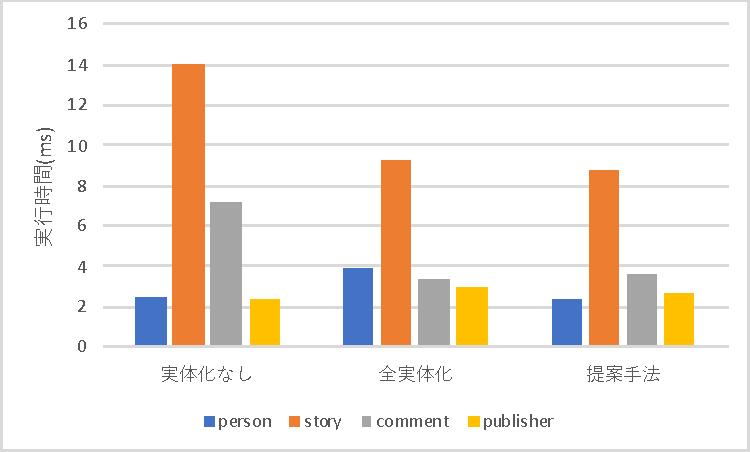
\includegraphics[width=30em]{src/ExperimentA-find.pdf} %[trim=left bottom right top]
	\end{center}
	\caption{実験Aの各コレクションの平均検索時間}
	\label{figure:ExperimentA-find}
\end{figure}
\begin{figure}[htbp]
	\begin{center}
		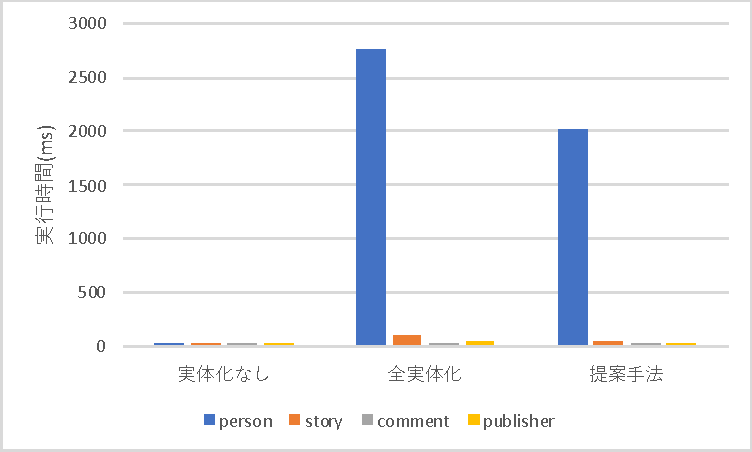
\includegraphics[width=30em]{src/ExperimentA-update.pdf} %[trim=left bottom right top]
	\end{center}
	\caption{実験Aの各コレクションの平均更新時間}
	\label{figure:ExperimentA-update}
\end{figure}
\begin{figure}[htbp]
	\begin{center}
		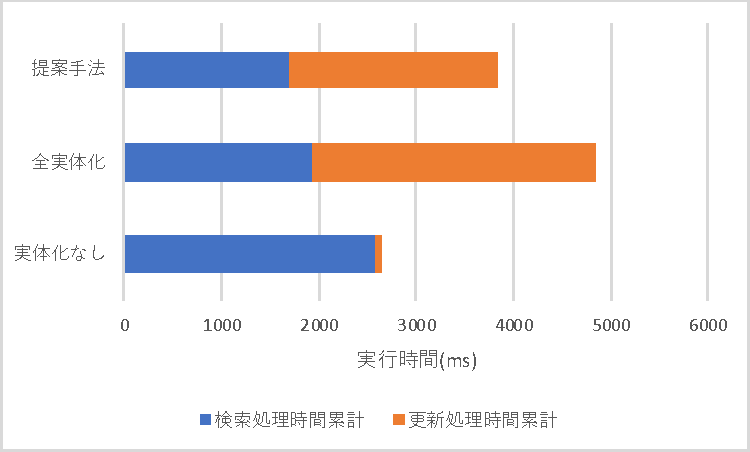
\includegraphics[width=30em]{src/ExperimentA-total.pdf} %[trim=left bottom right top]
	\end{center}
	\caption{実験Aの累計処理時間}
	\label{figure:ExperimentA-total}
\end{figure}

\section{実験Bの結果}
実験結果を図\ref{figure:ExperimentB-find},\ref{figure:ExperimentB-update},\ref{figure:ExperimentB-total}に示す.図\ref{figure:ExperimentB-find},\ref{figure:ExperimentB-update}は各コレクションにおけるクエリの平均処理時間を示している.図\ref{figure:ExperimentB-total}は検索処理と更新処理の累計処理時間を示している.全実体化と比べて提案手法は検索時間はさほど変わらないが,更新時間が半分程度となったため,累計処理時間で提案手がもっとも速い結果となった.
\begin{figure}[htbp]
	\begin{center}
		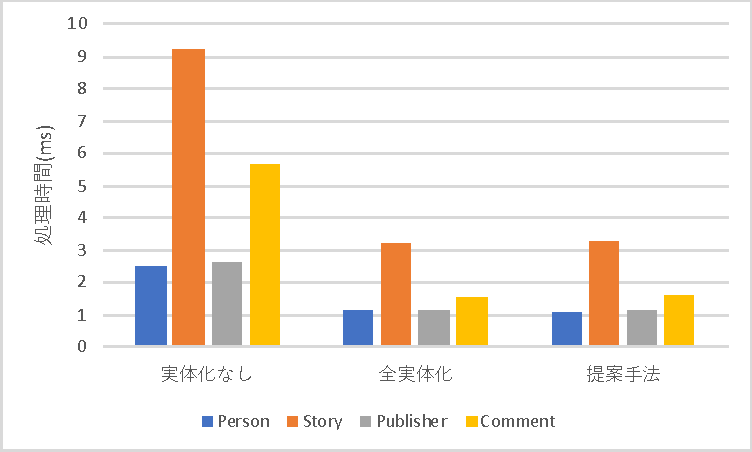
\includegraphics[width=30em]{src/ExperimentB-find.pdf} %[trim=left bottom right top]
	\end{center}
	\caption{実験Bの各コレクションの平均検索時間}
	\label{figure:ExperimentB-find}
\end{figure}
\begin{figure}[htbp]
	\begin{center}
		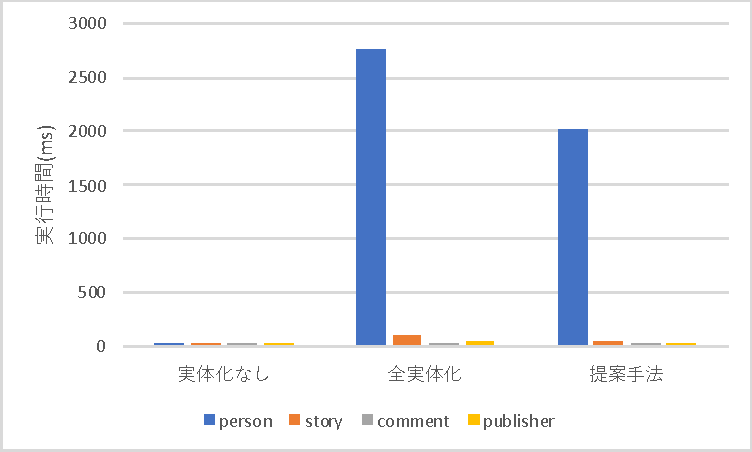
\includegraphics[width=30em]{src/ExperimentB-update.pdf} %[trim=left bottom right top]
	\end{center}
	\caption{実験Bの各コレクションの平均更新時間}
	\label{figure:ExperimentB-update}
\end{figure}
\begin{figure}[htbp]
	\begin{center}
		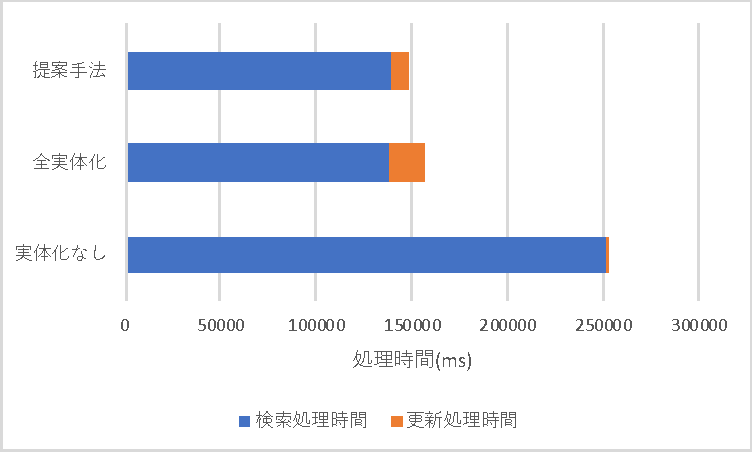
\includegraphics[width=30em]{src/ExperimentB-total.pdf} %[trim=left bottom right top]
	\end{center}
	\caption{実験Bの累計処理時間}
	\label{figure:ExperimentB-total}
\end{figure}

\section{実験Cの結果}
実験結果を図\ref{figure:ExperimentC-find},\ref{figure:ExperimentC-update},\ref{figure:ExperimentC-total}に示す.更新時間では提案手法が全実体化の半分程度だが,検索時間は全実体化の方が速く,累計処理時間は全実体化が一番速い結果となった.
\begin{figure}[htbp]
	\begin{center}
		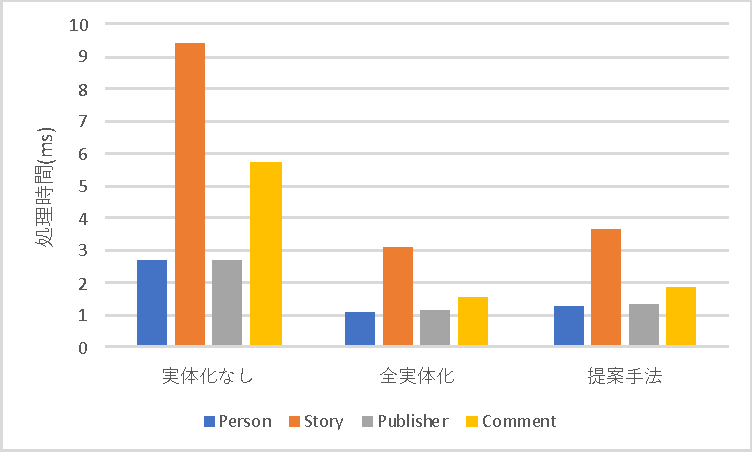
\includegraphics[width=30em]{src/ExperimentC-find.pdf} %[trim=left bottom right top]
	\end{center}
	\caption{実験Cの各コレクションの平均検索時間}
	\label{figure:ExperimentC-find}
\end{figure}
\begin{figure}[htbp]
	\begin{center}
		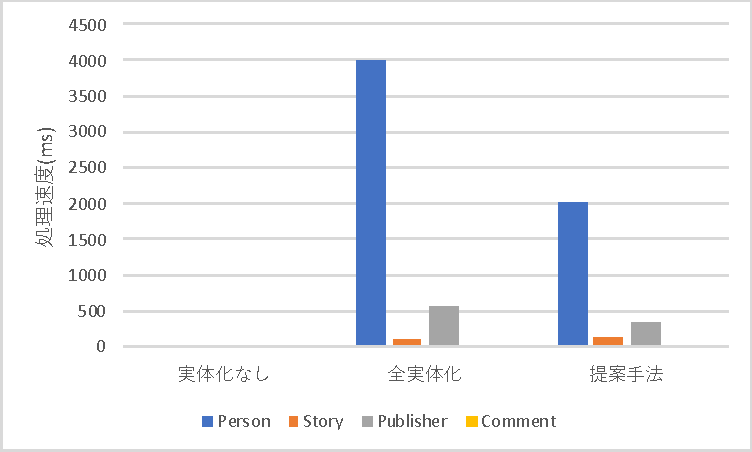
\includegraphics[width=30em]{src/ExperimentC-update.pdf} %[trim=left bottom right top]
	\end{center}
	\caption{実験Cの各コレクションの平均更新時間}
	\label{figure:ExperimentC-update}
\end{figure}
\begin{figure}[htbp]
	\begin{center}
		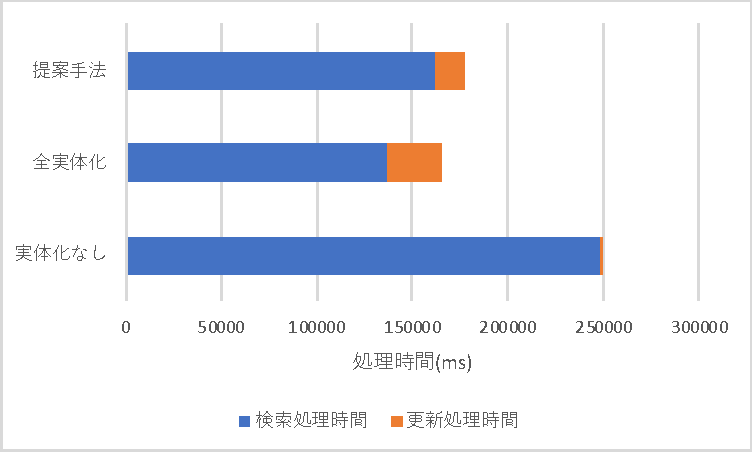
\includegraphics[width=30em]{src/ExperimentC-total.pdf} %[trim=left bottom right top]
	\end{center}
	\caption{実験Cの累計処理時間}
	\label{figure:ExperimentC-total}
\end{figure}

\section{実験Dの結果}
実験結果を図\ref{figure:ExperimentD-find},\ref{figure:ExperimentD-update},\ref{figure:ExperimentD-total}に示す.概ね実験Cと同じで,更新時間では全実体化と比べて提案手法の方が速いが,検索時間は全実体化の方が速く,累計処理時間では全実体化が一番速い結果となった.
\begin{figure}[htbp]
	\begin{center}
		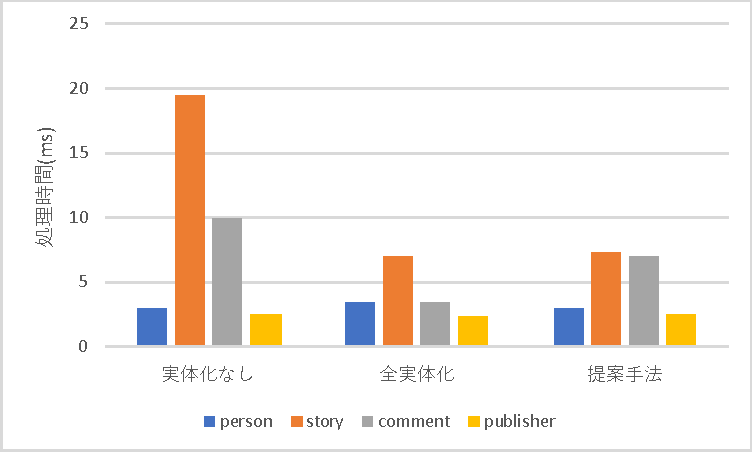
\includegraphics[width=30em]{src/ExperimentD-find.pdf} %[trim=left bottom right top]
	\end{center}
	\caption{実験Dの各コレクションの平均検索時間}
	\label{figure:ExperimentD-find}
\end{figure}
\begin{figure}[htbp]
	\begin{center}
		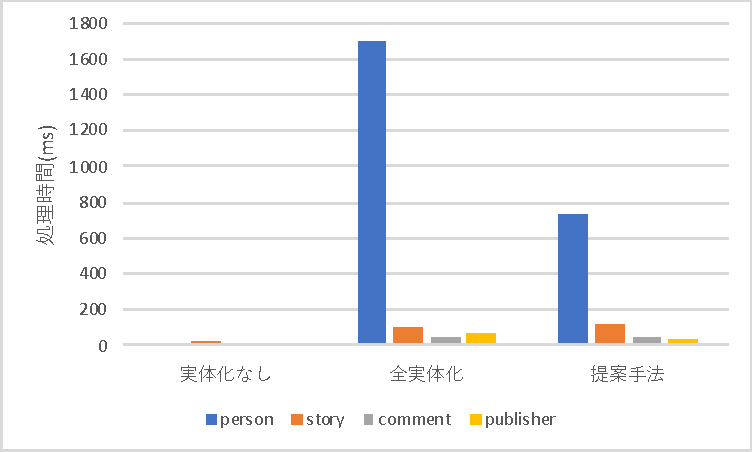
\includegraphics[width=30em]{src/ExperimentD-update.pdf} %[trim=left bottom right top]
	\end{center}
	\caption{実験Dの各コレクションの平均更新時間}
	\label{figure:ExperimentD-update}
\end{figure}
\begin{figure}[htbp]
	\begin{center}
		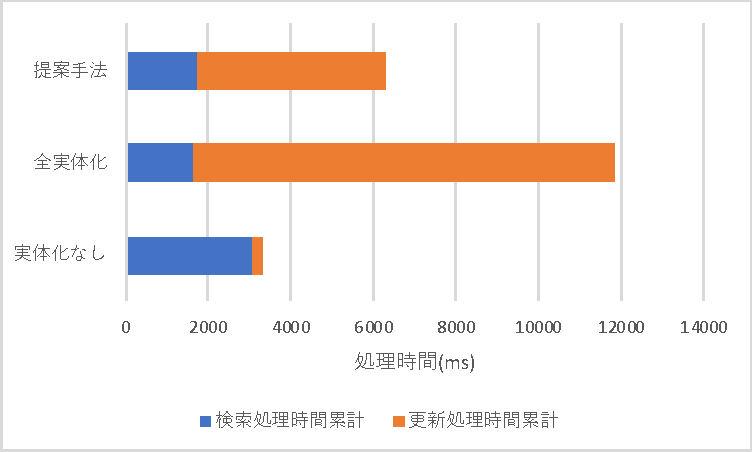
\includegraphics[width=30em]{src/ExperimentD-total.pdf} %[trim=left bottom right top]
	\end{center}
	\caption{実験Dの累計処理時間}
	\label{figure:ExperimentD-total}
\end{figure}

\section{実験Eの結果}
実験結果を図\ref{figure:ExperimentE-find},\ref{figure:ExperimentE-update},\ref{figure:ExperimentE-total}に示す.更新時間が全実体化と比べて提案手法2倍程度速い結果だが,検索時間は全実体化と比べて提案手法が1.2倍程遅く,累計処理時間では全実体化が最速という結果となった.
\begin{figure}[htbp]
	\begin{center}
		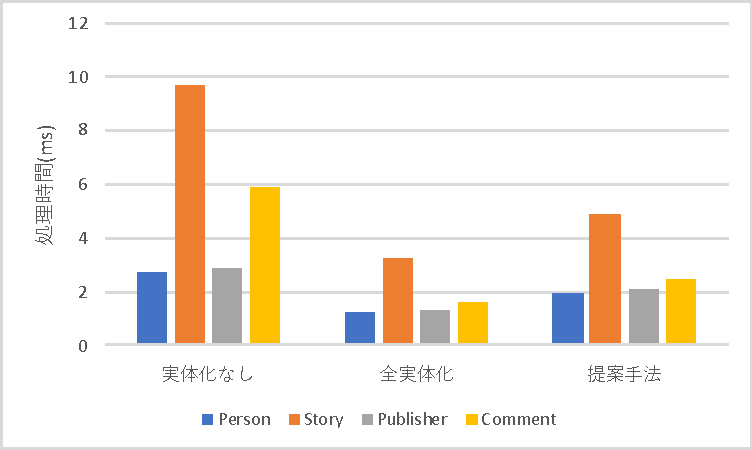
\includegraphics[width=30em]{src/ExperimentE-find.pdf} %[trim=left bottom right top]
	\end{center}
	\caption{実験Eの各コレクションの平均検索時間}
	\label{figure:ExperimentE-find}
\end{figure}
\begin{figure}[htbp]
	\begin{center}
		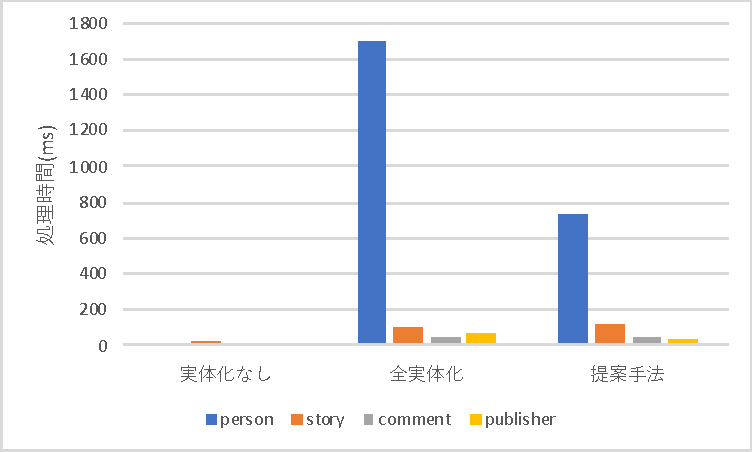
\includegraphics[width=30em]{src/ExperimentE-update.pdf} %[trim=left bottom right top]
	\end{center}
	\caption{実験Eの各コレクションの平均更新時間}
	\label{figure:ExperimentE-update}
\end{figure}
\begin{figure}[htbp]
	\begin{center}
		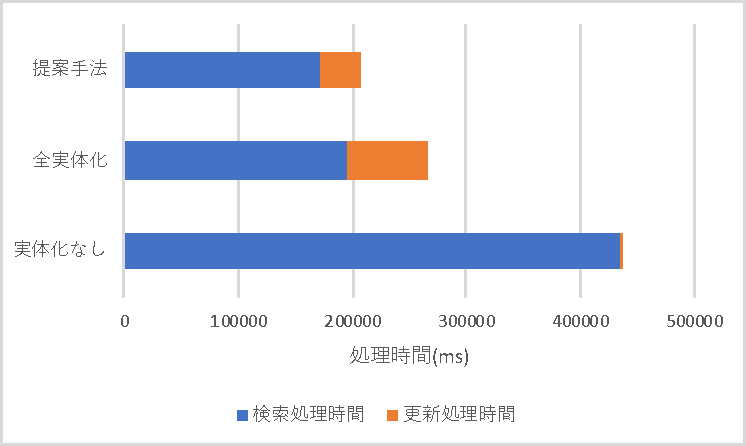
\includegraphics[width=30em]{src/ExperimentE-total.pdf} %[trim=left bottom right top]
	\end{center}
	\caption{実験Eの累計処理時間}
	\label{figure:ExperimentE-total}
\end{figure}

\section{実験Fの結果}
実験結果を図\ref{figure:ExperimentF-find},\ref{figure:ExperimentF-update},\ref{figure:ExperimentF-total}に示す.検索時間で全実体化が提案手法よりも1.5倍程度速く,更新時間で提案手法が全実体化と比べて2倍程度速い結果となった.累計処理時間では全実体化が最速となった.
\begin{figure}[htbp]
	\begin{center}
		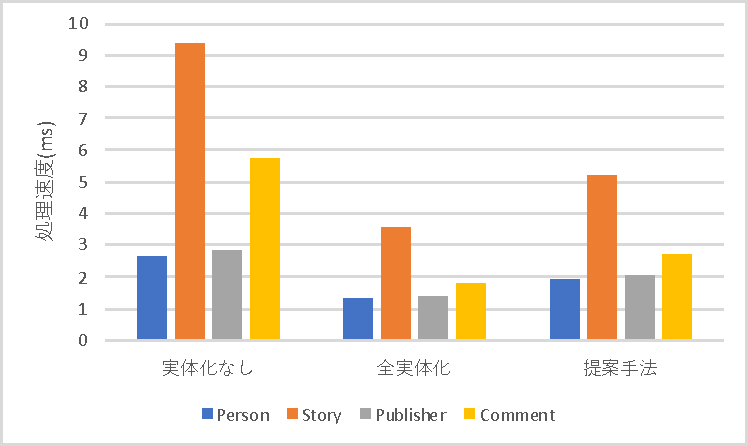
\includegraphics[width=30em]{src/ExperimentF-find.pdf} %[trim=left bottom right top]
	\end{center}
	\caption{実験Fの各コレクションの平均検索時間}
	\label{figure:ExperimentF-find}
\end{figure}
\begin{figure}[htbp]
	\begin{center}
		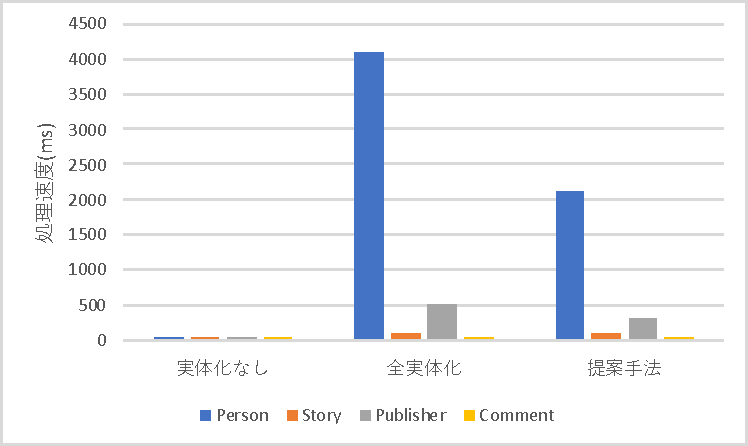
\includegraphics[width=30em]{src/ExperimentF-update.pdf} %[trim=left bottom right top]
	\end{center}
	\caption{実験Fの各コレクションの平均更新時間}
	\label{figure:ExperimentF-update}
\end{figure}
\begin{figure}[htbp]
	\begin{center}
		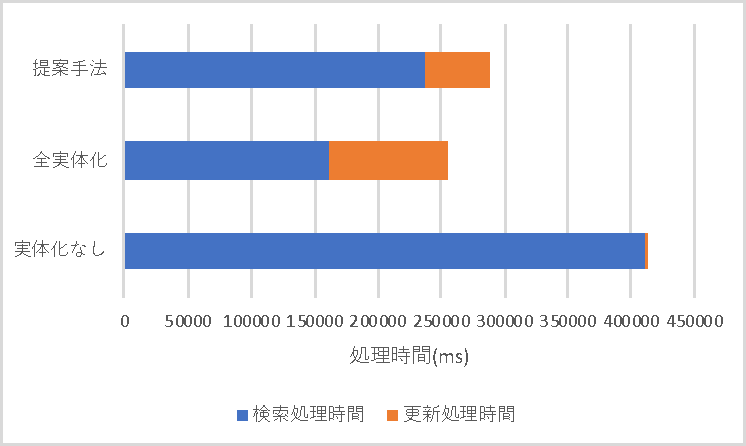
\includegraphics[width=30em]{src/ExperimentF-total.pdf} %[trim=left bottom right top]
	\end{center}
	\caption{実験Fの累計処理時間}
	\label{figure:ExperimentF-total}
\end{figure}

\section{実験Gの結果}
実験結果を図\ref{figure:ExperimentG-find},\ref{figure:ExperimentG-update},\ref{figure:ExperimentG-total}に示す.検索時間で全実体化が提案手法よりも1.2倍程度速く,更新時間で提案手法が全実体化と比べて2倍程度速い結果となった.累計処理時間では提案手法が最速となった.
\begin{figure}[htbp]
	\begin{center}
		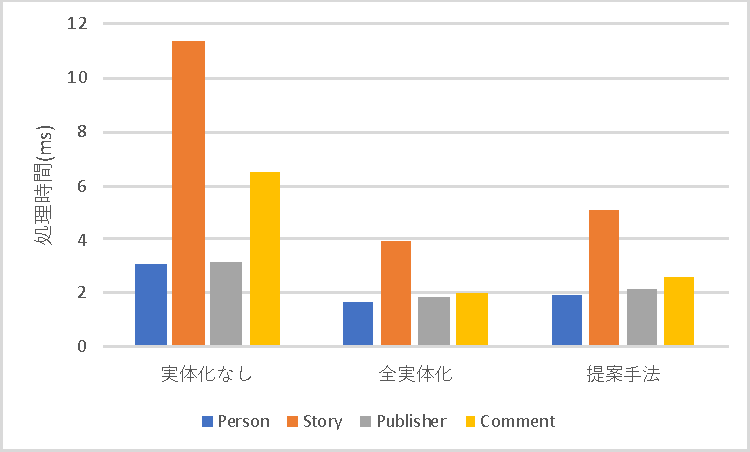
\includegraphics[width=30em]{src/ExperimentG-find.pdf} %[trim=left bottom right top]
	\end{center}
	\caption{実験Gの各コレクションの平均検索時間}
	\label{figure:ExperimentG-find}
\end{figure}
\begin{figure}[htbp]
	\begin{center}
		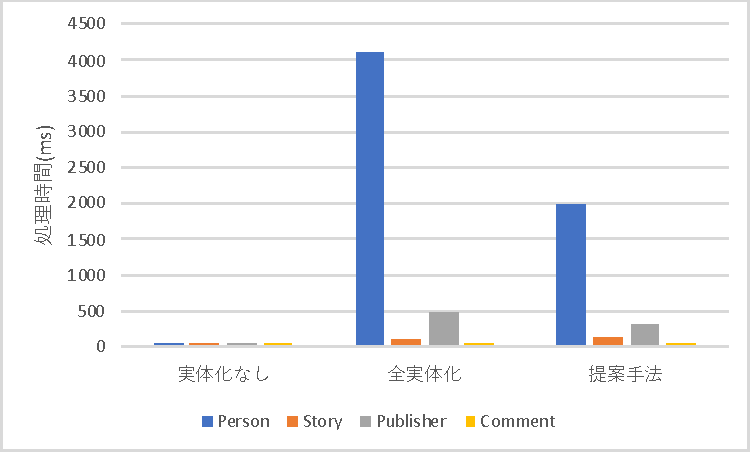
\includegraphics[width=30em]{src/ExperimentG-update.pdf} %[trim=left bottom right top]
	\end{center}
	\caption{実験Gの各コレクションの平均更新時間}
	\label{figure:ExperimentG-update}
\end{figure}
\begin{figure}[htbp]
	\begin{center}
		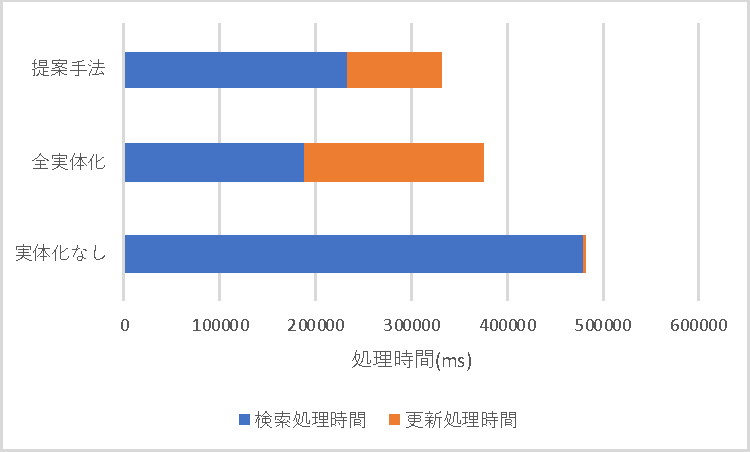
\includegraphics[width=30em]{src/ExperimentG-total.pdf} %[trim=left bottom right top]
	\end{center}
	\caption{実験Gの累計処理時間}
	\label{figure:ExperimentG-total}
\end{figure}

\section{実験Hの結果}
実験結果を図\ref{figure:ExperimentH-find},\ref{figure:ExperimentH-update},\ref{figure:ExperimentH-total}に示す.検索時間で全実体化が提案手法よりも1.2倍程度速く,更新時間で提案手法が全実体化と比べて2倍程度速い結果となった.累計処理時間では提案手法が最速となった.
\begin{figure}[htbp]
	\begin{center}
		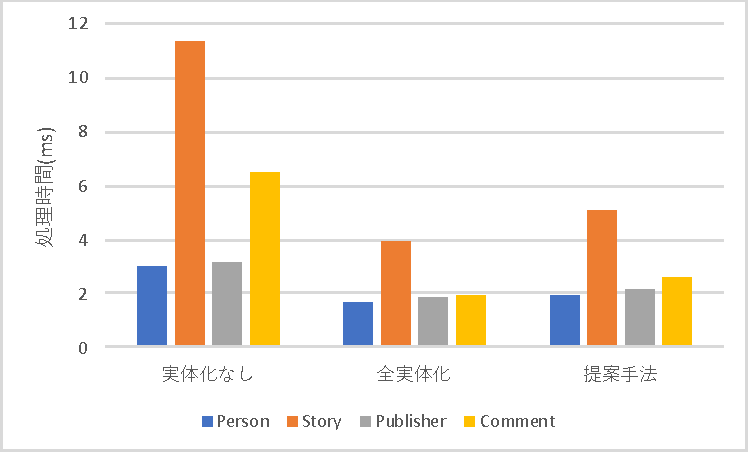
\includegraphics[width=30em]{src/ExperimentH-find.pdf} %[trim=left bottom right top]
	\end{center}
	\caption{実験Hの各コレクションの平均検索時間}
	\label{figure:ExperimentH-find}
\end{figure}
\begin{figure}[htbp]
	\begin{center}
		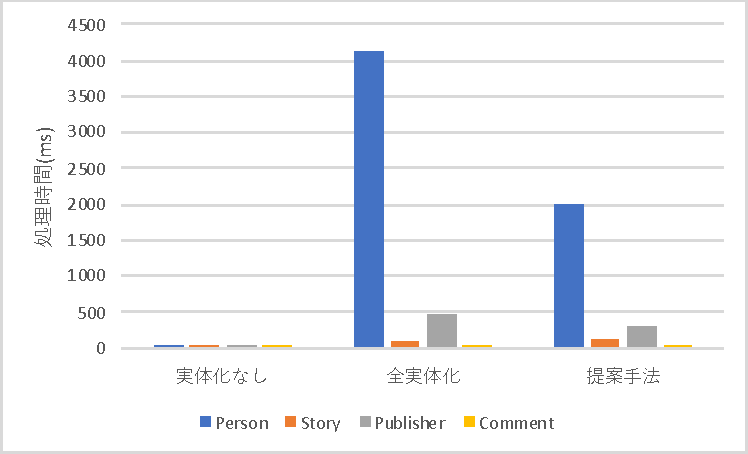
\includegraphics[width=30em]{src/ExperimentH-update.pdf} %[trim=left bottom right top]
	\end{center}
	\caption{実験Hの各コレクションの平均更新時間}
	\label{figure:ExperimentH-update}
\end{figure}
\begin{figure}[htbp]
	\begin{center}
		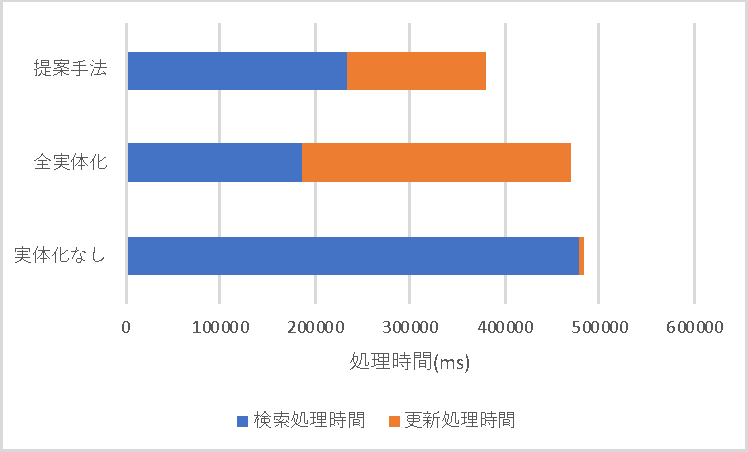
\includegraphics[width=30em]{src/ExperimentH-total.pdf} %[trim=left bottom right top]
	\end{center}
	\caption{実験Hの累計処理時間}
	\label{figure:ExperimentH-total}
\end{figure}

\section{実験の考察}
\label{sec:Consideration}

全実験において全実体化と提案手法は実体化なしと比べて累計検索処理時間が約半減した.通常であれば元のクエリに加えて結合先のクエリをMongoDB発行しアプリケーション層でドキュメントを結合するが,Materialized Viewを用いた場合には追加のクエリ発行と結合処理を省くことができる.その為,結合処理が発生するstory,commentコレクションの検索時間が高速化した.また,実体化した場合には更新時間が増大した.これはオリジナルのドキュメントに加えて,そのドキュメント自体のMaterialized Viewと,ドキュメントが埋め込まれているMaterialized Viewを更新する必要があり.MongoDB側に発行するクエリが増えるからである.今回の実験ではstoryコレクションに最大100のpersonドキュメントが埋め込まれており,personドキュメントを更新する際には実体化したpersonドキュメントと,そのドキュメントが埋め込まれているstoryドキュメントを更新する必要がある.実際に,実験Eではユーザーからのpersonコレクションへの9つのクエリに対してミドルウェアで521のクエリを発行していた.

実験AからFを通しての累計検索処理時間の推移を図\ref{figure:Experiment-find}に,累計更新処理時間の推移を図\ref{figure:Experiment-update}に,検索と更新を合わせた累計処理時間の推移を図\ref{figure:Experiment-total}に示す.

今回の実験ではupdateクエリ比が3\%以下の場合には実体化なしと比べて全実体化と提案手法が累計処理時間が速い結果となった.提案手法はupdateクエリ比が約1.4\%以上の際に全実体化と比べて累計処理時間が速いという結果となった.提案手法は想定通り全実体化と比べて更新処理時間を削減することができた.

図\ref{figure:Experiment-find}から分かるように,検索速度に関しては全実体化が最速である.全実体化と提案手法の検索処理時間の差はupdateクエリ比が1.0\%以降,ほぼ一定である.一方図\ref{figure:Experiment-update}から分かるように,updateクエリ比が増加するに比例して全実体化と提案手法の更新時間が増加するが,同様に全実体化と提案手法の差も増加する.この全実体化と提案手法の更新処理時間の差が検索処理時間の差を超えるupdateクエリ比が約1.4\%であり,これ以降累計処理時間で提案手法が最速となった.

\begin{figure}[htbp]
	\begin{center}
		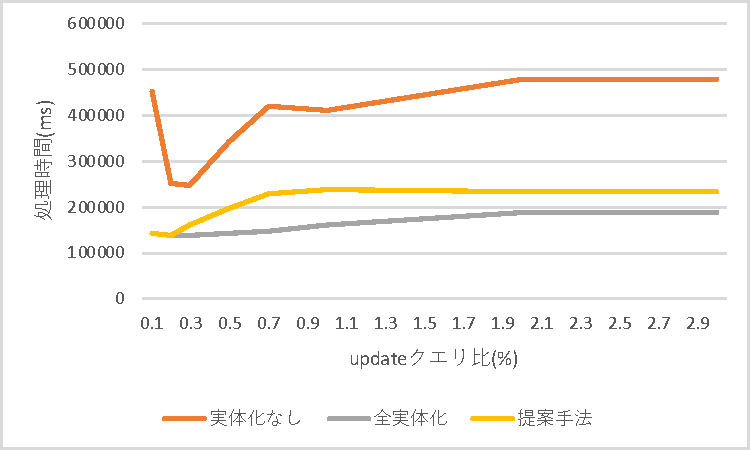
\includegraphics[width=30em]{src/Experiment-find.pdf} %[trim=left bottom right top]
	\end{center}
	\caption{累計検索処理時間の推移}
	\label{figure:Experiment-find}
\end{figure}
\begin{figure}[htbp]
	\begin{center}
		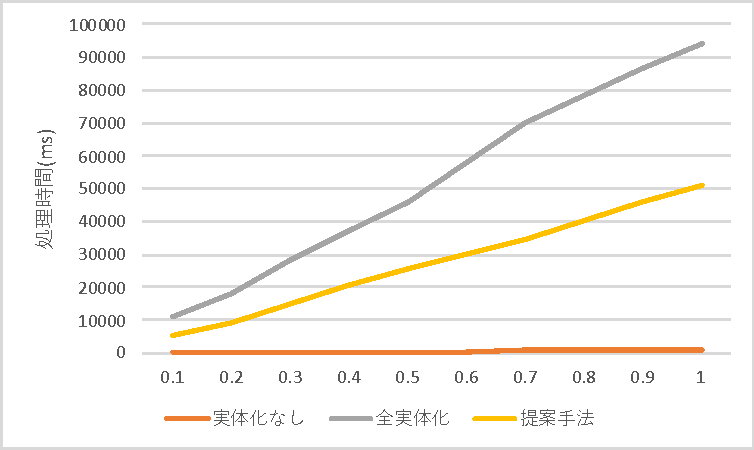
\includegraphics[width=30em]{src/Experiment-update.pdf} %[trim=left bottom right top]
	\end{center}
	\caption{累計更新処理時間の推移}
	\label{figure:Experiment-update}
\end{figure}
\begin{figure}[htbp]
	\begin{center}
		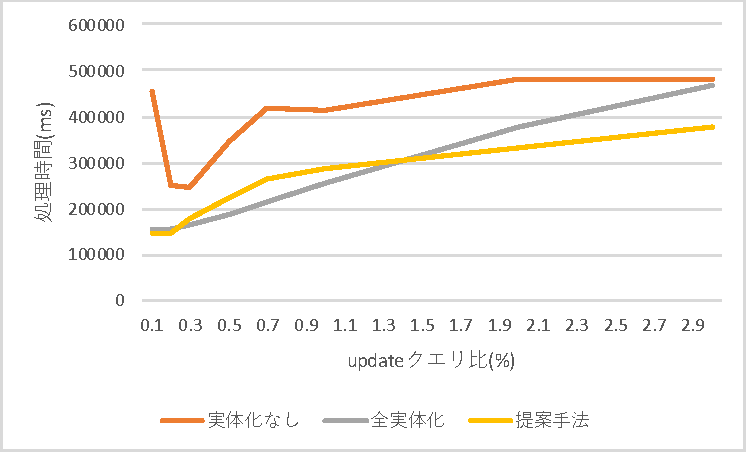
\includegraphics[width=30em]{src/Experiment-total.pdf} %[trim=left bottom right top]
	\end{center}
	\caption{累計処理時間の推移}
	\label{figure:Experiment-total}
\end{figure}


\end{document}
